\section{Implementation}
\labelsec{Implementation}
\subsection{Radar}
The console part of the radar is implemented as a web page, which is automatically generated in the \lstinline[columns=fixed]{srcMore} directory in a package associated with each Context when the \textbf{-httpserver} flag for a Context is set. It is implemented by a HTTP web-socket server working on port 8080. This interface emits different kind of events. For example, the Start button emits the event  \lstinline[columns=fixed]{cmd : cmd(start)}.
\begin{figure}[h]
	\centering
	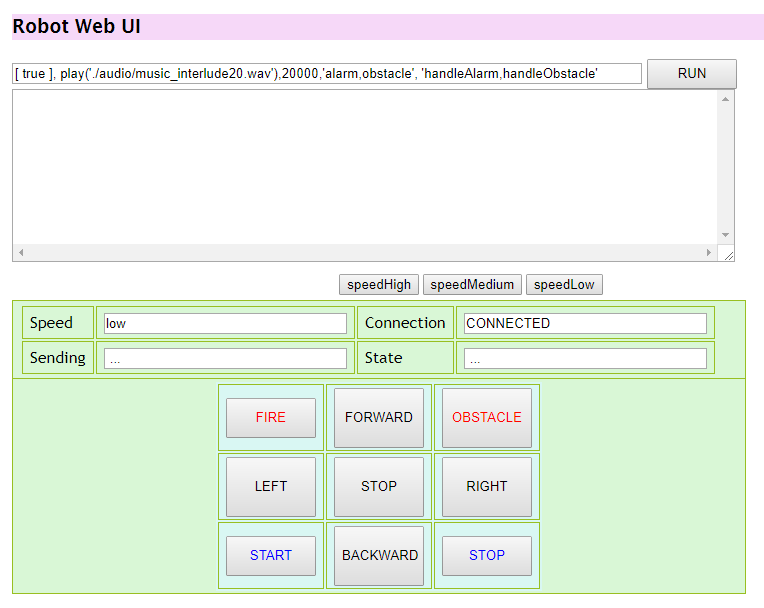
\includegraphics[width=\linewidth]{webconsole.png}
	\caption{Web console.}
\end{figure}
\\
The GUI part of the radar (where the sonars data are shown) is implemented using specific libraries provided by the software house.
\subsection{Led blinking}
The blink of the led has to be asynchronous, so that while the led is blinking, the robot can continue its operations without being blocked. In order to do so, the led is implemented as a \lstinline[columns=fixed]{SituatedActiveObject} supplied by the software house.
\lstinputlisting[style=java]{list/BlinkAsynch.java}
\subsection{Transmission of images through MQTT}
For the photo shoot through the camera, we used an open source library found on Github, called \textbf{JRPiCam} which wraps the commands needed to take a photo. Once the photo is acquired, it is converted in a String encoded with \textbf{Base64} encoding and then published on the \textbf{MQTT} broker, with a specified topic. The radar running on PC will have to decode the String received through MQTT in order to rebuild the image and then save it locally.
\lstinputlisting[style=java]{list/Camera.java}
\lstinputlisting[style=java]{list/Photoreceiver.java}